
\section{Results} \label{sec:results}
In this section, I present the results of the experiments and answer the two research questions. 
\subsection{RQ1 Results: CPD Performance}
\begin{sidewaystable} 
% \begin{table*}
\caption{Change point detection precision, recall, and F1-score calculated for the baseline methods using three values of tolerance ($\tau$) for multiple configurations.}
\label{tab:rq1-results}
\resizebox{\columnwidth}{!}{%
\begin{tabular}{llcccccccccc}
\toprule
  \textbf{Cost Function} &
  \textbf{Search Method} &
  \textbf{Penalty} &
  \textbf{Prec.} &
  \textbf{Recall} &
  \textbf{F1} &
  \textbf{Prec.} &
  \textbf{Recall} &
  \textbf{F1} &
  \textbf{Prec.} &
  \textbf{Recall} &
  \textbf{F1} \\
                                                  &              &   & \multicolumn{3}{c}{$\tau=1$s} & \multicolumn{3}{c}{$\tau=3$s} & \multicolumn{3}{c}{$\tau=5$s} \\  \toprule
\multirow{2}{*}{\textbf{Autoregressive Model}}     & Bottom Up    & 1000 & 10.43\%    & 75.44\%    & 18.33\%   & 21.21\%    & 80.32\%    & 33.55\%   & 28.94\%    & 81.22\%    & 42.68\%   \\
                                                   & Window Based & 100  & 2.94\%     & 3.98\%     & 3.38\%    & 8.53\%     & 11.41\%    & 9.76\%    & 12.89\%    & 17.54\%    & 14.86\%   \\ \midrule
\multirow{2}{*}{\textbf{Least Absolute Deviation}} & Bottom Up    & 500  & 7.32\%     & 52.54\%    & 12.85\%   & 17.52\%    & 87.73\%    & 29.20\%   & 25.02\%    & 88.95\%    & 39.05\%   \\
                                                   & Window Based & 500  & 5.24\%     & 8.31\%     & 6.42\%    & 15.20\%    & 24.03\%    & 18.62\%   & 21.79\%    & 38.25\%    & 27.76\%   \\ \midrule
\multirow{2}{*}{\textbf{Least Squared Deviation}}  & Bottom Up    & 1000 & 7.44\%     & 85.09\%    & 13.68\%   & 16.40\%    & 89.81\%    & 27.74\%   & 24.16\%    & 90.47\%    & 38.14\%   \\
                                                   & Window Based & 500  & 3.59\%     & 6.79\%     & 4.70\%    & 10.27\%    & 16.51\%    & 12.66\%   & 16.18\%    & 26.84\%    & 20.19\%   \\ \midrule
\multirow{2}{*}{\textbf{Linear Model Change}}      & Bottom Up    & 100  & \textbf{37.59\%}    & 28.98\%    & \textbf{32.73\%}   & \textbf{45.20\%}    & 38.39\%    & \textbf{41.52\%}   & \textbf{48.07\%}    & 41.36\%    & \textbf{44.46\% }  \\
                                                   & Window Based & 500  & 6.70\%     & 4.14\%     & 5.12\%    & 20.50\%    & 13.05\%    & 15.95\%   & 38.78\%    & 26.77\%    & 31.67\%   \\ \midrule
\multirow{2}{*}{\textbf{Gaussian Process Change}}  & Bottom Up    & 100  & 3.77\%     & \textbf{92.23\%}    & 7.25\%    & 8.99\%     & \textbf{92.23\%}    & 16.39\%   & 13.53\%    & \textbf{92.23\%}    & 23.60\%   \\
                                                   & Window Based & 100  & 2.94\%     & 3.95\%     & 3.37\%    & 8.69\%     & 11.50\%    & 9.90\%    & 13.64\%    & 18.30\%    & 15.63\%   \\ \midrule
\multirow{2}{*}{\textbf{Rank-based Cost Function}} & Bottom Up    & 100  & 13.45\%    & 60.19\%    & 21.98\%   & 19.49\%    & 80.10\%    & 31.35\%   & 22.98\%    & 87.23\%    & 36.38\%   \\
                                                   & Window Based & 100  & 8.10\%     & 13.70\%    & 10.18\%   & 15.72\%    & 30.73\%    & 20.80\%   & 21.38\%    & 46.64\%    & 29.32\%   \\ \midrule
\multirow{2}{*}{\textbf{Kernelized Mean Change}}   & Bottom Up    & 100  & 4.13\%     & 3.24\%     & 3.63\%    & 12.22\%    & 8.14\%     & 9.77\%    & 15.38\%    & 10.58\%    & 12.54\%   \\
                                                   & Window Based & 100  & 2.82\%     & 3.00\%     & 2.91\%    & 10.14\%    & 8.40\%     & 9.19\%    & 13.64\%    & 12.61\%    & 13.10\%   \\ \bottomrule

                                                   
\end{tabular}%
}
% \end{table*}
\end{sidewaystable}

Table~\ref{tab:rq1-results} shows the results of running CPD algorithms for various configurations (as described in \ref{sec:CPD_baseline}). For each search method and cost function pair only one of the penalty values which resulted in the highest F1 scores for all $\tau$ values is reported. 

The first observation from the results is that as values of $\tau$ increases the scores get better. This was expected, since larger values relax the constraints on which detected change points are considered as a true positive. Another observation is that the bottom-up segmentation consistently outperforms the window-based segmentation method. I can also see that the linear cost function beats all the other ones, in terms of precision. The Gaussian cost function achieves much higher recall values costing it a huge loss in precision. It means this cost function results in detecting numerous change points spread across the time axis, so there is a good chance of having at least one change point predicted close to each true change point (hence the high recall), but also there are a lot of false positives, which leads to a low precision. 

\begin{table}
\caption{Change point detection precision, recall, and F1-score calculated, on the test data, for the proposed model, using three values of tolerance ($\tau$) compared with the respective $\tau$'s best F1 score among baseline methods}
\label{tab:rq1-2-results}
% begin{tabular}{cccc}
\begin{tabularx}{\columnwidth}{cXXXX}
\toprule
  $\mathbf{\tau}$ &
  \textbf{Prec.} &
  \textbf{Recall} &
  \textbf{F1 score} & 
  \textbf{Baseline F1}  \\ \midrule
1s & 56.77\% &	79.32\% &	66.18\% & 32.73\% \\
3s & 69.58\% &	88.88\% &	78.06\% & 41.52\% \\
5s & 79.82\% &	91.87\%	&   85.42\% & 44.46\% \\\bottomrule
\end{tabularx}
%\end{tabular}
\end{table}

Measuring the same metrics on how the proposed model performs on the test data shows better scores, almost twice the F1 score of the best performing baseline (see Table~\ref{tab:rq1-2-results}). 
Please note that unlike machine learning algorithms (such as mine), CPD algorithms do not have a separate training and testing phases. This fact works in their favor (by using the entire dataset for prediction and not just the training set), but still my model outperforms them.

%Although measuring the time it takes to detect change points was not one of the comparison metrics it would not hurt to note that
In terms of execution cost, running all 42 different settings of CPD algorithms on the whole dataset took a bit over 12 hours in the cloud using 16 CPUs and 64GB of main memory. The deep learning model on the other hand takes about an hour to train (which only needs to be done once), on a smaller machine (see section~\ref{sec:machines_config}). It made predictions on the whole dataset in less than a minute.
%$(/)-1=
So to answer RQ1, my method has shown $(66.18/32.73)-1=102.20\%$ improvement in F1 score with $\tau=1s$, $(78.06/41.52)-1=88.00\%$ with $\tau=3s$, and $(85.42/44.46)-1=92.13\%$ with $\tau=5s$; almost doubling the score compared to the baselines. 

\begin{rqanswer}
The proposed model, which requires less memory compared to traditional CPD algorithms, improved their best performance by up to 102\%, measured by F1 score, in less execution time.
\end{rqanswer}

\subsection{RQ2 Results: Multi-class Classification Performance}
To answer RQ2, I first compare different configurations of the baseline methods using the F1 score (harmonic mean of precision and recall) on the test data. The results are presented in Table~\ref{tab:rq2-1-results}.

\begin{table}
\caption{Precision, recall, and F1 score of ridge classifiers (linear classifiers with L2 regularization) and decision tree classifiers (DT) with different sliding window widths ($w$). For each algorithm on each $w$ several hyper-parameters were applied producing 152 different models. In this table, I only show the results of the best performing model in each group.}
\label{tab:rq2-1-results}
\resizebox{\linewidth}{!}{%
\begin{tabular}{clcclll}
\toprule
\textbf{w} &
  \multicolumn{1}{c}{\textbf{Classifier}} &
  \multicolumn{1}{c}{\textbf{\begin{tabular}[c]{@{}c@{}}Max\\ Depth\end{tabular}}} &
  \multicolumn{1}{c}{\textbf{\begin{tabular}[c]{@{}c@{}}Max\\ Features\end{tabular}}} &
  \multicolumn{1}{c}{\textbf{Prec.}} &
  \multicolumn{1}{c}{\textbf{Recall}} &
  \multicolumn{1}{c}{\textbf{F1}} \\ \midrule
3  & Ridge & -   & -          & 71.39\% & 20.73\% & 32.13\% \\
3  & DT    & -   & -          & 69.21\% & 82.36\% & 75.21\% \\ \midrule
5  & Ridge & -   & -          & 69.15\% & 21.89\% & 33.26\% \\
5  & DT    & 100 & -          & 68.37\% & \textbf{83.16\%} & 75.04\% \\ \midrule
10 & Ridge & -   & -          & 71.97\% & 24.02\% & 36.02\% \\
10 & DT    & 260 & -          & 67.94\% & 79.14\% & 73.12\% \\ \midrule
15 & Ridge & -   & -          & 76.87 & 25.90\% & 38.75\% \\
15 & DT    & -   & $\sqrt{10w}$ & 69.06\% & 80.76\% & 74.45\% \\ \midrule
20 & Ridge & -   & -          & \textbf{80.38\%} & 26.50\% & 39.86\% \\
20 & DT    & 175 & $\sqrt{10w}$ & 73.21\% & 82.16\% & \textbf{77.42\%} \\  \midrule
   & \multicolumn{3}{l}{My Approach} & \textbf{86.29\%} & \textbf{95.04\%} & \textbf{90.45\%} \\
\bottomrule
\end{tabular}%
}
\end{table}

Comparing the baseline methods with my approach (the last row) in Table~\ref{tab:rq2-1-results} shows that my model outperforms all baselines. Comparing it with the model with the best F1-score shows a $(86.29/73.21)-1=17.87\%$ improvement in precision as well as a $(95.04/82.16)-1=15.68\%$ improvement in recall that means $(90.45/77.42)-1=16.83\%$ overall improvement in F1-score. 

To have a feeling of how good my predictions are in practice, Figure~\ref{fig:test_0} shows the output of my model side by side with the ground truth. The horizontal axis shows sample ID (time) and the states are color coded. As it is seen, this algorithm performs better when the state changes are farther apart. Also there are some state changes that happen quite briefly which are not detected. That is not to a great surprise since it takes some time for state changes to be reflected in the outputs and those might not have got any chance.


The classical models only see one window of the data at a time, convolutional layers on the other hand are more generalized and flexible since each filter in each layer is comparable to a sliding window. As you saw in Table~\ref{tab:rq2-1-results}, a larger window size means a higher performance. However, it gets significantly more difficult to train a model with large window sizes. In addition, convolutions can automatically learn preprocessing steps that could be beneficial such as a moving average. Each convolutional filter can learn a linear combination of its inputs. So when the convolutional layers are stacked on each other, with non-linear activation functions in between, the hypothesis space they can learn becomes quite large, probably much larger than most of the classical ML algorithms here. Also, they are still quite efficient (more efficient than baselines) due to parameter sharing and their high parallelizability.

The fact that the performance improves as the window size increases indicates the positive effect of being able to see longer-term relations in detecting the system's state. Recurrent cells (such as GRU) can capture long-term dependencies (that do not necessarily fall into one window) and learn sequences. This is one of the major differences between an RNN model and others, such as decision trees, which do not have such a notion of a ``long-term memory'' as LSTM/GRU neural networks do. All a decision tree could see is the values in a sliding window.

In terms of the training complexity (time and memory), this method is superior as well. That can largely be attributed to the use of deep learning. In baseline models, as the window size $w$ grows the training and evaluation complexity grows, up to a point that they ran out of memory -- consuming all the 47GB of main memory and swap area. This forced us to train them in the cloud. Meanwhile, as mentioned earlier, the deep learning model could be trained on a 8GB GPU in roughly an hour. (see section \ref{sec:machines_config} for the machines' specs). Also, the decision tree training was not parallelized using only one core of the CPU, while virtually all deep learning models can be heavily parallelized on a GPU/TPU. %All the reported scores for both the baseline models and my model are computed on previously unseen test data. 

\begin{rqanswer}
The proposed model, which requires less than half as many CPUs and 70\% as much memory compared to the best performing classical ML model, improved their best performance by up to 17\%, measured by F1 score, in less execution time.
\end{rqanswer}


\begin{figure*}
    \centering
    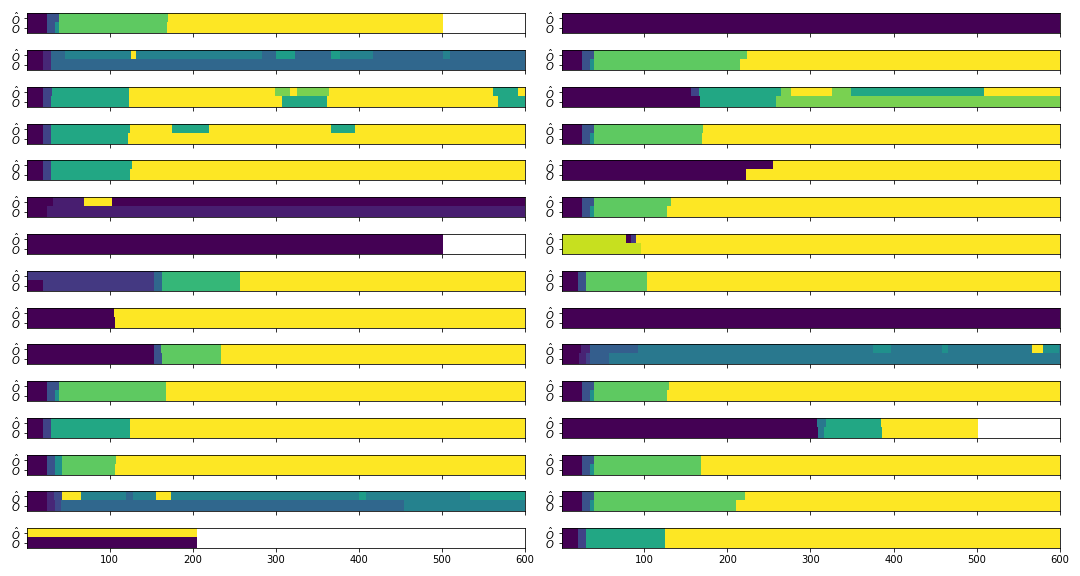
\includegraphics[width=\linewidth]{ASE_files/test_0.png}
    % \Description[States in time diagram]{A figure that color-codes the true and predicted states}
    \caption{Evaluation of the model on 30 random test data. Each graph shows the states in one run of the system. The colors show the states. The top-half of each plot depicts model's prediction of the system states ($\hat{O}$) and the bottom-half shows the true labels($O$). Since the output is one-hot encoded, the item with the most probability is used as the predicted label at each point in time. X-axis is the time axis. Only the first 600 samples (2 minute of simulation) are shown to improve legibility.}
    \label{fig:test_0}
\end{figure*}

\subsection{RQ3 Results: CPD Performance on Paparazzi (replication)}
\hl{NEW SECTION}
The results of applying baseline algorithms on Paparazzi data set can be seen in table~\ref{tab:cpd_paparazzi}.
The numbers are quite varied, for example there are scores worse then 1\% as well as some 100\% recall scores. 
The 100\% recalls are accompanied with a low precision; achieving that is not difficult. A method that outputs every point as a change-point will get similar results. 
The setting that got most of the best numbers is Pelt algorithm using an L1 cost function and a high penalty coefficient of 1000. However, please note that Pelt is a quite slow algorithm that could easily become infeasible to run on larger data set, as it was the case for the first two RQs. 
As a matter of fact, running Pelt took more than 14 hours on the same machine that performed all other CPD algorithms in less than 1 hour. What you see in table~\ref{tab:cpd_paparazzi} is the summary of the results of more than 23800 experiments. 

Comparing the baseline results with the neural network model's results in the last three rows of the table, you can see improvements of 48.9\%, 26.83\%, and 11.46\% in F1 scores compared to the best numbers in the baselines (for $\tau = 1, 3, 5$ seconds respectively). Although this model still performed better than the baselines, the improvement margin was higher in RQ1. (see the RQ1 results summary box and the paragraph above that). % in section~\ref{sec:results}). 
However, you can see that the scores that this approach achieved are not low, but the baselines could do a better job on Paparazzi's data compared to MicroPilot's, therefore shrinking the margin of improvement. 
It can be due to the fact that the new data set is tiny compared to MP, classic machine learning algorithms can do better so a deep learning model cannot shine here as it could for MP. 
As a reminder: Paparazzi data set consists of ~300 tests vs. ~900 tests in MP, and simulation lengths are up to 2500 samples vs. 18000 in MP's data set. 
It is worth mentioning that both in the first two RQs and here, the variation in baselines performances was way higher while my deep learning approach shows a more consistent performance; check the second column (recall with $\tau=1$s) for example. 

\begin{rqanswer}
The proposed approach was applied on another similar software system with a smaller data set size and showed a near 49\% improvement over the baselines, confirming that it is a feasible approach even with smaller data set size. The lower margin of improvement compared to RQ1 is attributed to the baselines performing better on this data, rather than my approach not performing good enough.
\end{rqanswer}

\begin{sidewaystable}
    \centering
\resizebox{\columnwidth}{!}{%
\begin{tabular}{llcccccccccc}
\toprule
  \textbf{Cost Function} &
  \textbf{Search Method} &
  \textbf{Penalty} &
  \textbf{Prec.} &
  \textbf{Recall} &
  \textbf{F1} &
  \textbf{Prec.} &
  \textbf{Recall} &
  \textbf{F1} &
  \textbf{Prec.} &
  \textbf{Recall} &
  \textbf{F1} \\
                                                  &              &   & \multicolumn{3}{c}{$\tau=1$s} & \multicolumn{3}{c}{$\tau=3$s} & \multicolumn{3}{c}{$\tau=5$s} \\  \toprule
\multirow{3}{*}{\textbf{Autoregressive Model}}
    & bottomup & 500  &       13.65\% &    14.13\% & 18.89\% &        39.73\% &     36.40\% & 36.14\% &        57.11\% &     53.20\% & 50.04\% \\
    & exact & 500  &       13.56\% &    13.85\% & 19.03\% &        39.67\% &     36.17\% & 36.03\% &        56.97\% &     52.89\% & 49.83\% \\
    & window & 100  &       15.97\% &     7.59\% & 13.54\% &        45.47\% &     20.40\% & 29.56\% &        64.16\% &     30.76\% & 41.20\% \\ \midrule
\multirow{3}{*}{\textbf{Least Absolute Deviation}}
    & window & 100  &       24.50\% &    15.92\% & 19.85\% &        56.39\% &     37.24\% & 44.53\% &        68.94\% &     48.20\% & 56.23\% \\
    & exact & 1000 &       \textbf{26.74\%} &    34.08\% & 29.92\% &        \textbf{60.77\%} &     77.32\% & \textbf{67.74\%} &        \textbf{74.73\%} &     93.16\% & \textbf{82.61\%} \\
    & bottomup & 1000 &       26.66\% &\textbf{34.99\%}& 30.35\% &        60.11\% &     78.14\% & 67.61\% &        72.85\% &     92.94\% & 81.30\% \\ \midrule
\multirow{3}{*}{\textbf{Least Squared Deviation}}
    & window & 1000 &       25.01\% &    16.14\% & 20.26\% &        54.58\% &     35.77\% & 42.96\% &        68.73\% &     48.11\% & 56.18\% \\
    & exact & 1000 &       21.28\% &    80.04\% & 33.49\% &        51.05\% &     99.58\% & 67.20\% &        65.36\% & \textbf{99.97\%} & 78.76\% \\
    & bottomup & 1000 &       21.30\% &    81.24\% & \textbf{33.62\%} &        50.98\% &\textbf{99.50\%}& 67.12\% &        65.24\% &\textbf{99.97\%}& 78.66\% \\ \midrule
\multirow{3}{*}{\textbf{Linear Model Change}}
    & bottomup & 100  &        7.39\% &     0.39\% &  9.98\% &        27.44\% &      1.49\% & 10.27\% &        52.51\% &      2.75\% &  9.90\% \\
    & window & 100  &        7.39\% &     0.39\% &  9.98\% &        27.44\% &      1.49\% & 10.27\% &        52.51\% &      2.75\% &  9.90\% \\
    & exact & 100  &        7.39\% &     0.39\% &  9.98\% &        27.44\% &      1.49\% & 10.27\% &        52.51\% &      2.75\% &  9.90\% \\ \midrule
\multirow{3}{*}{\textbf{Gaussian Process Change}}
    & window & 100  &        7.39\% &     0.39\% &  9.98\% &        27.44\% &      1.49\% & 10.27\% &        52.51\% &      2.75\% &  9.90\% \\
    & exact & 100  &        7.39\% &     0.39\% &  9.98\% &        27.44\% &      1.49\% & 10.27\% &        52.51\% &      2.75\% &  9.90\% \\
    & bottomup & 100  &       12.42\% &   \textbf{100.00\%} & 22.03\% &        33.15\% &    \textbf{100.00\%} & 49.55\% &        49.04\% &    \textbf{100.00\%} & 65.47\% \\ \midrule
\multirow{2}{*}{\textbf{Rank-based Cost Function}}
    & exact & 100  &       21.11\% &    31.85\% & 25.51\% &        52.29\% &     74.63\% & 61.13\% &        65.88\% &     89.30\% & 75.46\% \\
    & bottomup & 100  &       20.55\% &    31.84\% & 25.17\% &        49.97\% &     73.22\% & 59.04\% &        64.57\% &     89.35\% & 74.61\% \\ \midrule
\multirow{3}{*}{\textbf{Kernelized Mean Change}} 
    & bottomup & 100  &       15.66\% &     1.90\% &  9.45\% &        44.23\% &      5.36\% & 12.95\% &        62.37\% &      7.48\% & 15.66\% \\
    & exact & 100  &       14.07\% &     1.64\% &  9.77\% &        42.06\% &      4.74\% & 12.59\% &        60.92\% &      6.67\% & 14.56\% \\
    & window & 100  &        8.31\% &     0.61\% &  9.97\% &        29.38\% &      2.02\% & 10.60\% &        53.34\% &      3.39\% & 10.79\% \\ \midrule \midrule
\multirow{3}{*}{\textbf{My Approach}} 
    & \multirow{3}{*}{\textbf{Data set:}}  
         & \textbf{Validation} &  45.63\% &    55.46\% & 50.07\% &   81.39\% &     90.97\% & 85.92\% &   88.38\% &     97.12\% & 92.54\%  \\
    & {} & b\textbf{Test (Tuning)} &  42.65\% &    54.87\% & 47.99\% &   76.73\% &     90.96\% & 83.24\% &   85.18\% &     97.46\% & 90.91\%  \\
    & {} & \textbf{Training}  &  39.81\% &    51.96\% & 45.08\% &   75.69\% &     90.62\% & 82.49\% &   84.96\% &     97.55\% & 90.82\%  \\
\bottomrule
\end{tabular}%
}
    \caption{Change point detection methods performance on Paparazzi data set. Since the 100\% recalls are actually outliers, the next largest recall values are in bold face as well.}
    \label{tab:cpd_paparazzi}
\end{sidewaystable}

\subsection{RQ4 Results: Multi-class Classification Performance on Paparazzi (replication)}
\hl{NEW SECTION}
In table~\ref{tab:rq2-1-results-replicate} the comparative results of the aforementioned algorithms with my method is presented. 
To compare with the MP's case, we can see that in all but two settings limiting the maximum number of features did not help improve the model. 
Another similar observation is that the scores do not vary much with changing the window size, and decision trees almost universally outperform linear classifiers.
The scores themselves are just around the same values as well: Ridge classifier F1 score here is in 21-29\% range, which was 32-39\% in RQ2. For decision trees it is in 67-68\% range here while it is in 73-77\% range in RQ 2. 

The deep learning model's performance measures (on validation data) can be found in the last row of the table. 
You can see an $(81.92-68.96)-1=18.79\%$ improvement in F1 score, over the baselines. It confirms that this method can beat the best performing baselines in classifying input samples into the system's internal states. The improvement in RQ2 is 16.83\%, not very different from this. This, again confirms the reproducibility of the results in the first two RQs.

\begin{table}
\caption{Precision, recall, and F1 score of ridge classifiers (linear classifiers with L2 regularization) and decision tree classifiers with different sliding window widths ($w$). In this table, I only show the results of the best performing model in each group.}
\label{tab:rq2-1-results-replicate}
\resizebox{\linewidth}{!}{%
\begin{tabular}{llcccc}
\toprule
\textbf{w} &
  \multicolumn{1}{c}{\textbf{Classifier}} &
  \multicolumn{1}{c}{\textbf{Max Features}} &
  \multicolumn{1}{c}{\textbf{Precision}} &
  \multicolumn{1}{c}{\textbf{Recall}} &
  \multicolumn{1}{c}{\textbf{F1}} \\ \midrule
 3 &  Ridge &            - &      44.82\% &   14.45\% & 21.85\% \\
 3 & Decision Tree & $\sqrt{10w}$ &      61.88\% &   73.56\% & 67.22\% \\ \midrule
 5 &  Ridge &            - &      46.62\% &   15.10\% & 22.81\% \\
 5 & Decision Tree &            - &      64.28\% &   73.00\% & 68.36\% \\ \midrule
10 &  Ridge &            - &      47.59\% &   16.29\% & 24.27\% \\
10 & Decision Tree &            - &\textbf{65.06\%}& 73.36\% &\textbf{68.96\%}\\ \midrule
15 &  Ridge &            - &      44.41\% &   17.33\% & 24.93\% \\
15 & Decision Tree &            - &      63.53\% &   74.68\%& 68.65\% \\ \midrule
20 &  Ridge &            - &      57.97\% &   19.10\% & 28.74\% \\
20 & Decision Tree &            - &      64.72\% &   73.36\% & 68.77\% \\ \midrule
25 &  Ridge &            - &      62.13\% &   19.66\% & 29.87\% \\
25 & Decision Tree & $\sqrt{10w}$ &      61.17\% &\textbf{75.18}\% & 67.45\% \\ \midrule \midrule
   & \multicolumn{2}{l}{Proposed Method} & \textbf{71.13\%} & \textbf{88.69\%} & \textbf{81.92\%} \\
\bottomrule
\end{tabular}%
}
\end{table}

They say a picture is worth a thousand words\footnote{missing citation}, to better see the predictions of the deep learning model compared to the ground truth, see figure~\ref{fig:paparazzi_predictions}. 
\begin{figure}
    \centering
    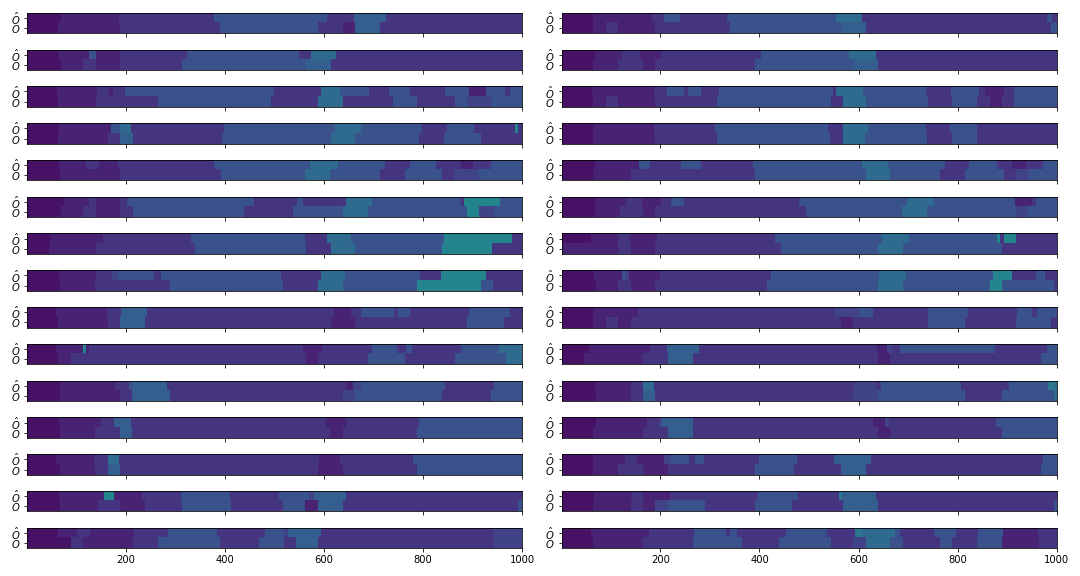
\includegraphics[width=\columnwidth]{RQ3-5_charts/states_chart.png}
    \caption{The states are color coded and each rectangle shows one test, only the first 1000 samples (200 seconds) are shown for more clarity. The same as figure~\ref{fig:test_0} in, the top half of each rectangle shows the model's output and the bottom half shows the true labels.}
    \label{fig:paparazzi_predictions}
\end{figure}


\begin{rqanswer}
Compared to the baselines, the proposed approach could detect the internal state of system with a 71\% precision and 89\% recall rate, showing a 19\% improvements. Similar results were seen in RQ 2 (which is closely related to this question) confirming that the improvements are replicable and are not just a fluke.
\end{rqanswer}

\subsection{RQ5 Results: Hyper-parameter Tuning}
\hl{NEW SECTION}
I used Tensor Board to visualize and compare the effects of different hyper-parameters on the model's performance. First, for a sanity check, I visualized 4 metrics, precision and recall in detecting change points with a small tolerance of $\tau=1s$, and precision and recall in estimating the internal state. A healthy linear and positive correlation is visible between all pairs of these metrics, it means that trying to improve one usually will not come at the expense of others. 
\begin{figure}
    \centering
    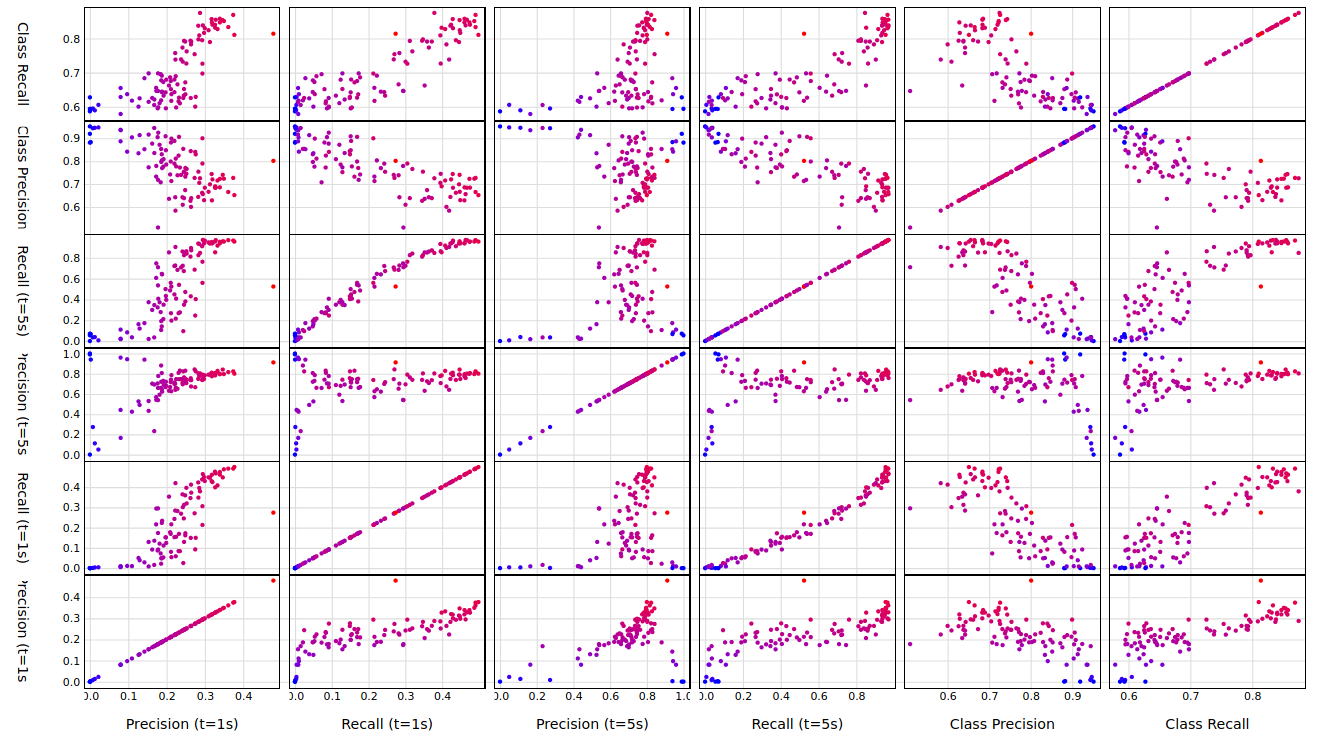
\includegraphics[width=\columnwidth]{RQ3-5_charts/prec_recall_matrix_tuning_white_background.png}
    \caption{Matrix of scatter plots comparing precision and recall of the deep learning model on test data.}
    \label{fig:precision_recall_matrix}
\end{figure}

Filtering the data to find the commonalities of better hyper-parameters shows that the number of GRU cells has a high correlation with both CPD precision and classification precision. 
It also shows that the kernel sizes and number of convolutional layers does not have an as strong correlation with higher precision and recalls. The number of convolutional filters in each layer has a bigger impact on the performance than the size of the kernels does. 
It makes sense because training larger kernels gets harder and harder and requires more data. Also, based on the previous studies, especially in the field of computer vision, we can say that each filter learns one feature so it is more effective to have many small filters that are easier to train and can learn multiple features of the data.
Therefore I can reduce the size of convolutional section of the model and use more recurrent cells to boost the performance without adding too many parameters. I performed another set of tests in a smaller search space to further optimize the hyper-parameters.

The new search space was all the combinations of these hyper-parameters:

\begin{enumerate}
    \item Learning rate, options being: $3\times10^{-4}$, $1\times10^{-3}$, and $3\times10^{-3}$
    \item Number of GRU cells, options: 128, 256, 384, and 512
    \item Number of convolutional filters in each layer: 32, 64, and 72
\end{enumerate}

\begin{figure}
    \centering
    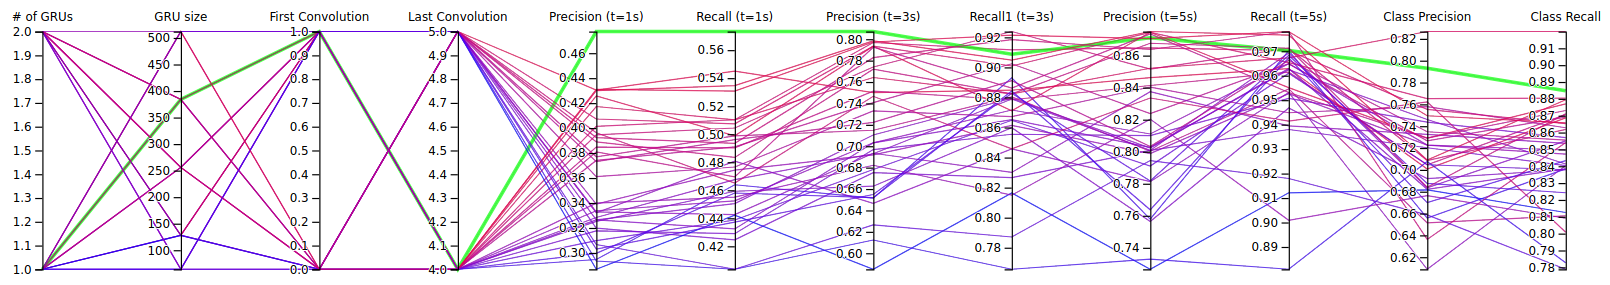
\includegraphics[width=\columnwidth]{RQ3-5_charts/refined_prec_recall_white_background.png}
    \caption{Parallel coordinates view showing the effects of select hyper-parameters on the performance measures.}
    \label{fig:precision_recall_parallel_coordinates}
\end{figure}
The results of the second round of tuning are shown in figure~\ref{fig:precision_recall_parallel_coordinates}. This chart shows 3 + 8 parallel axis, 3 hyper-parameters and 8 metrics. To make it more legible, the results with lower than 70\% precision ($\tau = 5s$) are omitted.
The green highlighted line is the best configuration tried, with the highest area under the curve. That configuration has the best or close to the best performance in all metrics. The configuration is to use 256 GRU cells, 72 filter per layer, and the lower learning rate of $3\times10^{-4}$.

I used these hyper-parameters to train the best model. The scores used in the research question 3 and 4 are the evaluation results of this model on the [previously unseen] validation data. The stopping criteria on training the model was for the validation loss to plateau, with a `patience' of 15 epochs. The optimizer converged in 54 epochs, after less than 3 minutes of training. 

\begin{rqanswer}
The result of this tuning was a model with fewer convolutional layers and smaller kernel sizes but with more convolutional filters and recurrent layers that could perform better than the baselines. This shows having more and smaller convolutional filters is more effective in capturing local features in the data compared to having a small number of large filters (with kernels of size 20 for example which has 200 parameters). It also shows the important role that recurrent layers play in discovering long-term relations between inputs and outputs. 
\end{rqanswer}


\section{Limitations and Threats to Validity} \label{sec:threats_to_validity}
One of the limitations of this approach is that it might miss an input-output invariant correlation. It can happen when the input remains constant or it changes too little to reveal its relation with certain outputs. 
%In addition, as mentioned before, my approach relies on changes in signals. 
The assumption is that during the data collection, sampling happens in regular intervals; this approach probably will have a hard time achieving high performances, working on unevenly spaced time-series data.
%Maybe the CPD baselines could perform better if they were boosted by feature engineering, but the feature engineering task is can quickly become an arduous and inefficient. 
%It exists so it compensates for inability of traditional non-deep-learning methods in discovering meaningful features in the data. \cite{bengio2013deep}

In terms of construct validity, I am using standard metrics to evaluate the results. However, the use of tolerance margin should be taken with caution since it is a domain-dependant variable and can change the final results. To alleviate this threats, I have used multiple margins and reported all results. In terms of internal validity threats, I reduced the threat by not implementing the CPD baselines by myself and rather reusing existing libraries. In terms of conclusion validity threats, I have used many (888) real test cases from Micropilot's test repository and provided a proper train-validation-test split for training, tuning, and evaluation. \hl{Finally, in terms of external validity threats, this study suffers from being limited to only one case study. However, the study is a large-scale real-world study with many test cases. I plan to extend this work with more case studies from other domains, to increase its generalizability.}

